\documentclass{extbook}[14pt]
\usepackage{multicol, enumerate, enumitem, hyperref, color, soul, setspace, parskip, fancyhdr, amssymb, amsthm, amsmath, bbm, latexsym, units, mathtools}
\everymath{\displaystyle}
\usepackage[headsep=0.5cm,headheight=0cm, left=1 in,right= 1 in,top= 1 in,bottom= 1 in]{geometry}
\usepackage{dashrule}  % Package to use the command below to create lines between items
\newcommand{\litem}[1]{\item #1

\rule{\textwidth}{0.4pt}}
\pagestyle{fancy}
\lhead{}
\chead{Answer Key for Progress Quiz 10 Version C}
\rhead{}
\lfoot{}
\cfoot{}
\rfoot{Fall 2020}
\begin{document}
\textbf{This key should allow you to understand why you choose the option you did (beyond just getting a question right or wrong). \href{https://xronos.clas.ufl.edu/mac1105spring2020/courseDescriptionAndMisc/Exams/LearningFromResults}{More instructions on how to use this key can be found here}.}

\textbf{If you have a suggestion to make the keys better, \href{https://forms.gle/CZkbZmPbC9XALEE88}{please fill out the short survey here}.}

\textit{Note: This key is auto-generated and may contain issues and/or errors. The keys are reviewed after each exam to ensure grading is done accurately. If there are issues (like duplicate options), they are noted in the offline gradebook. The keys are a work-in-progress to give students as many resources to improve as possible.}

\rule{\textwidth}{0.4pt}

\begin{enumerate}\litem{
Simplify the expression below into the form $a+bi$. Then, choose the intervals that $a$ and $b$ belong to.
\[ \frac{-72 - 11 i}{-4 + 3 i} \]
The solution is \( 10.20  + 10.40 i \), which is option A.\begin{enumerate}[label=\Alph*.]
\item \( a \in [9.5, 12] \text{ and } b \in [10, 12] \)
* $10.20  + 10.40 i$, which is the correct option.
\item \( a \in [9.5, 12] \text{ and } b \in [259, 260.5] \)
 $10.20  + 260.00 i$, which corresponds to forgetting to multiply the conjugate by the numerator.
\item \( a \in [17.5, 19] \text{ and } b \in [-4, -2.5] \)
 $18.00  - 3.67 i$, which corresponds to just dividing the first term by the first term and the second by the second.
\item \( a \in [12, 13.5] \text{ and } b \in [-7, -6] \)
 $12.84  - 6.88 i$, which corresponds to forgetting to multiply the conjugate by the numerator and not computing the conjugate correctly.
\item \( a \in [254, 255.5] \text{ and } b \in [10, 12] \)
 $255.00  + 10.40 i$, which corresponds to forgetting to multiply the conjugate by the numerator and using a plus instead of a minus in the denominator.
\end{enumerate}

\textbf{General Comment:} Multiply the numerator and denominator by the *conjugate* of the denominator, then simplify. For example, if we have $2+3i$, the conjugate is $2-3i$.
}
\litem{
Simplify the expression below into the form $a+bi$. Then, choose the intervals that $a$ and $b$ belong to.
\[ (8 - 9 i)(10 + 3 i) \]
The solution is \( 107 - 66 i \), which is option C.\begin{enumerate}[label=\Alph*.]
\item \( a \in [77, 82] \text{ and } b \in [-30, -23] \)
 $80 - 27 i$, which corresponds to just multiplying the real terms to get the real part of the solution and the coefficients in the complex terms to get the complex part.
\item \( a \in [53, 56] \text{ and } b \in [-117, -113] \)
 $53 - 114 i$, which corresponds to adding a minus sign in the second term.
\item \( a \in [106, 118] \text{ and } b \in [-70, -58] \)
* $107 - 66 i$, which is the correct option.
\item \( a \in [53, 56] \text{ and } b \in [106, 118] \)
 $53 + 114 i$, which corresponds to adding a minus sign in the first term.
\item \( a \in [106, 118] \text{ and } b \in [66, 68] \)
 $107 + 66 i$, which corresponds to adding a minus sign in both terms.
\end{enumerate}

\textbf{General Comment:} You can treat $i$ as a variable and distribute. Just remember that $i^2=-1$, so you can continue to reduce after you distribute.
}
\litem{
Simplify the expression below and choose the interval the simplification is contained within.
\[ 5 - 11 \div 16 * 8 - (6 * 7) \]
The solution is \( -42.500 \), which is option A.\begin{enumerate}[label=\Alph*.]
\item \( [-43.2, -40.6] \)
* -42.500, which is the correct option.
\item \( [-39.8, -37] \)
 -37.086, which corresponds to an Order of Operations error: not reading left-to-right for multiplication/division.
\item \( [-47.3, -43.9] \)
 -45.500, which corresponds to not distributing a negative correctly.
\item \( [46.1, 49.7] \)
 46.914, which corresponds to not distributing addition and subtraction correctly.
\item \( \text{None of the above} \)
 You may have gotten this by making an unanticipated error. If you got a value that is not any of the others, please let the coordinator know so they can help you figure out what happened.
\end{enumerate}

\textbf{General Comment:} While you may remember (or were taught) PEMDAS is done in order, it is actually done as P/E/MD/AS. When we are at MD or AS, we read left to right.
}
\litem{
Choose the \textbf{smallest} set of Complex numbers that the number below belongs to.
\[ \sqrt{\frac{630}{5}}+\sqrt{165} i \]
The solution is \( \text{Nonreal Complex} \), which is option B.\begin{enumerate}[label=\Alph*.]
\item \( \text{Not a Complex Number} \)
This is not a number. The only non-Complex number we know is dividing by 0 as this is not a number!
\item \( \text{Nonreal Complex} \)
* This is the correct option!
\item \( \text{Rational} \)
These are numbers that can be written as fraction of Integers (e.g., -2/3 + 5)
\item \( \text{Pure Imaginary} \)
This is a Complex number $(a+bi)$ that \textbf{only} has an imaginary part like $2i$.
\item \( \text{Irrational} \)
These cannot be written as a fraction of Integers. Remember: $\pi$ is not an Integer!
\end{enumerate}

\textbf{General Comment:} Be sure to simplify $i^2 = -1$. This may remove the imaginary portion for your number. If you are having trouble, you may want to look at the \textit{Subgroups of the Real Numbers} section.
}
\litem{
Choose the \textbf{smallest} set of Real numbers that the number below belongs to.
\[ \sqrt{\frac{1190}{5}} \]
The solution is \( \text{Irrational} \), which is option E.\begin{enumerate}[label=\Alph*.]
\item \( \text{Rational} \)
These are numbers that can be written as fraction of Integers (e.g., -2/3)
\item \( \text{Whole} \)
These are the counting numbers with 0 (0, 1, 2, 3, ...)
\item \( \text{Not a Real number} \)
These are Nonreal Complex numbers \textbf{OR} things that are not numbers (e.g., dividing by 0).
\item \( \text{Integer} \)
These are the negative and positive counting numbers (..., -3, -2, -1, 0, 1, 2, 3, ...)
\item \( \text{Irrational} \)
* This is the correct option!
\end{enumerate}

\textbf{General Comment:} First, you \textbf{NEED} to simplify the expression. This question simplifies to $\sqrt{238}$. 
 
 Be sure you look at the simplified fraction and not just the decimal expansion. Numbers such as 13, 17, and 19 provide \textbf{long but repeating/terminating decimal expansions!} 
 
 The only ways to *not* be a Real number are: dividing by 0 or taking the square root of a negative number. 
 
 Irrational numbers are more than just square root of 3: adding or subtracting values from square root of 3 is also irrational.
}
\end{enumerate}

\end{document}\documentclass{extbook}[14pt]
\usepackage{multicol, enumerate, enumitem, hyperref, color, soul, setspace, parskip, fancyhdr, amssymb, amsthm, amsmath, bbm, latexsym, units, mathtools}
\everymath{\displaystyle}
\usepackage[headsep=0.5cm,headheight=0cm, left=1 in,right= 1 in,top= 1 in,bottom= 1 in]{geometry}
\usepackage{dashrule}  % Package to use the command below to create lines between items
\newcommand{\litem}[1]{\item #1

\rule{\textwidth}{0.4pt}}
\pagestyle{fancy}
\lhead{}
\chead{Answer Key for Progress Quiz 10 Version C}
\rhead{}
\lfoot{}
\cfoot{}
\rfoot{Fall 2020}
\begin{document}
\textbf{This key should allow you to understand why you choose the option you did (beyond just getting a question right or wrong). \href{https://xronos.clas.ufl.edu/mac1105spring2020/courseDescriptionAndMisc/Exams/LearningFromResults}{More instructions on how to use this key can be found here}.}

\textbf{If you have a suggestion to make the keys better, \href{https://forms.gle/CZkbZmPbC9XALEE88}{please fill out the short survey here}.}

\textit{Note: This key is auto-generated and may contain issues and/or errors. The keys are reviewed after each exam to ensure grading is done accurately. If there are issues (like duplicate options), they are noted in the offline gradebook. The keys are a work-in-progress to give students as many resources to improve as possible.}

\rule{\textwidth}{0.4pt}

\begin{enumerate}\litem{
Write the equation of the line in the graph below in Standard form $Ax+By=C$. Then, choose the intervals that contain $A, B, \text{ and } C$.

\begin{center}
    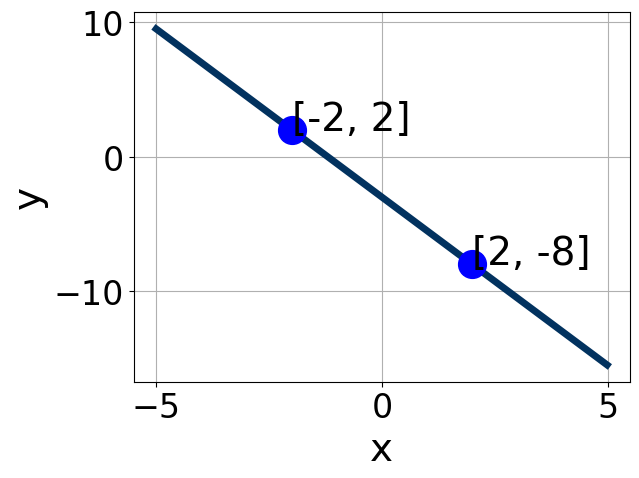
\includegraphics[width=0.5\textwidth]{../Figures/linearGraphToStandardC.png}
\end{center}

The solution is \( 4x + 5y = 15 \), which is option A.\begin{enumerate}[label=\Alph*.]
\item \( A \in [3, 5], \hspace{3mm} B \in [4.3, 6.84], \text{ and } \hspace{3mm} C \in [13, 17] \)
* $4x + 5y = 15$, which is the correct option.
\item \( A \in [0.8, 1.8], \hspace{3mm} B \in [0.67, 1.34], \text{ and } \hspace{3mm} C \in [2, 7] \)
 $0.8x + 1y = 3.0$, which corresponds to not removing rational values for Standard Form.
\item \( A \in [3, 5], \hspace{3mm} B \in [-5.94, -4.52], \text{ and } \hspace{3mm} C \in [-18, -5] \)
 $4x - 5y = -15$, which corresponds to using the opposite (negative) slope of the graph, but did everything else correctly.
\item \( A \in [0.8, 1.8], \hspace{3mm} B \in [-1.22, -0.94], \text{ and } \hspace{3mm} C \in [-3, -2] \)
 $0.8x - 1y = -3.0$, which corresponds to using the opposite (negative) slope of the graph and not removing rational values.
\item \( A \in [-6, 0], \hspace{3mm} B \in [-5.94, -4.52], \text{ and } \hspace{3mm} C \in [-18, -5] \)
 $-4x - 5y = -15$, which corresponds to not making $A$ positive (by multiplying the equation by $-1$).
\end{enumerate}

\textbf{General Comment:} Standard form is supposed to have $A > 0$ and all fractions removed.
}
\litem{
Find the equation of the line described below. Write the linear equation as $ y=mx+b $ and choose the intervals that contain $m$ and $b$.
\[ \text{Perpendicular to } 7 x - 6 y = 15 \text{ and passing through the point } (-4, -9). \]
The solution is \( y = -0.86x - 12.43 \), which is option A.\begin{enumerate}[label=\Alph*.]
\item \( m \in [-0.9, -0.61] \hspace*{3mm} b \in [-13.27, -12.32] \)
* $y = -0.86x - 12.43$, which is the correct option.
\item \( m \in [-0.9, -0.61] \hspace*{3mm} b \in [-5.44, -4.75] \)
 $y = -0.86x - 5.00$, which corresponds to correct slope and mis-distributing while simplifying to slope-intercept form.
\item \( m \in [0.71, 1.43] \hspace*{3mm} b \in [-6.03, -5.21] \)
 $y = 0.86x - 5.57$, which corresponds to using the negative slope.
\item \( m \in [-1.64, -1.14] \hspace*{3mm} b \in [-13.27, -12.32] \)
 $y = -1.17x - 12.43$, which corresponds to using the reciprocal slope $(1/m)$.
\item \( m \in [-0.9, -0.61] \hspace*{3mm} b \in [12.18, 13.19] \)
 $y = -0.86x + 12.43$, which corresponds to using the correct slope and getting the negative $y$-intercept.
\end{enumerate}

\textbf{General Comment:} Parallel slope is the same and perpendicular slope is opposite reciprocal. Opposite reciprocal means flipping the fraction and changing the sign (positive to negative or negative to positive).
}
\litem{
First, find the equation of the line containing the two points below. Then, write the equation as $ y=mx+b $ and choose the intervals that contain $m$ and $b$.
\[ (4, 3) \text{ and } (3, 10) \]
The solution is \( y = -7.0x + 31.0 \), which is option E.\begin{enumerate}[label=\Alph*.]
\item \( m \in [-13, -3] \hspace*{3mm} b \in [2, 10] \)
 $y = -7.0x + 7$, which corresponds to using the correct slope/equation but not distributing correctly using the second point.
\item \( m \in [-13, -3] \hspace*{3mm} b \in [-39, -26] \)
 $y = -7.0x -31.0$, which corresponds to using the correct slope and getting the negative y-intercept.
\item \( m \in [-13, -3] \hspace*{3mm} b \in [-3, 3] \)
 $y = -7.0x -1$, which corresponds to using the correct slope/equation but not distributing correctly using the first point.
\item \( m \in [7, 11] \hspace*{3mm} b \in [-12, -10] \)
 $y = 7.0x -11.0$, which corresponds to using the negative slope and the correct equation.
\item \( m \in [-13, -3] \hspace*{3mm} b \in [31, 32] \)
* $y = -7.0x + 31.0$, which is the correct option.
\end{enumerate}

\textbf{General Comment:} Remember to keep your points in order when plugging in to the slope formula.
}
\litem{
Solve the equation below. Then, choose the interval that contains the solution.
\[ -13(2x + 6) = -14(8x -12) \]
The solution is \( x = -4.176 \), which is option D.\begin{enumerate}[label=\Alph*.]
\item \( x \in [-1.13, -0.99] \)
* $x = -1.021$, which corresponds to getting the negative of the actual solution.
\item \( x \in [-0.91, -0.68] \)
* $x = -0.747$, which corresponds to not distributing the negative in front of the first parentheses correctly.
\item \( x \in [5.35, 5.78] \)
* $x = 5.706$, which corresponds to not distributing the negative in front of the second parentheses correctly.
\item \( x \in [-4.5, -3.91] \)
* $x = -4.176$, which is the correct option.
\item \( \text{There are no real solutions.} \)
Corresponds to students thinking a fraction means there is no solution to the equation.
\end{enumerate}

\textbf{General Comment:} The most common mistake on this question is to not distribute the negative in front of the second fraction correctly. The best way to avoid this is putting the numerator in parentheses, which will help you remember to distribute the negative correctly.
}
\litem{



\textbf{General Comment:} None
}
\litem{
Solve the linear equation below. Then, choose the interval that contains the solution.
\[ \frac{3x + 5}{4} - \frac{4x -7}{7} = \frac{6x -9}{5} \]
The solution is \( x = 3.965 \), which is option C.\begin{enumerate}[label=\Alph*.]
\item \( x \in [-0.3, 1.2] \)
 $x = 0.579$, which corresponds to dividing the second number in the numerator by the denominator rather than dividing BOTH parts of the numerator by the denominator (or removing the fractions through multiplication).
\item \( x \in [20.3, 22.3] \)
 $x = 20.559$, which corresponds to dividing the coefficients in front of x by the denominator rather than dividing BOTH parts of the numerator by the denominator (or removing the fractions through multiplication).
\item \( x \in [3.2, 4.2] \)
* $x = 3.965$, which is the correct option.
\item \( x \in [0.7, 2.7] \)
 $x = 2.007$, which corresponds to not distributing the negative in front of the second fraction.
\item \( \text{There are no real solutions.} \)
Corresponds to students thinking a fraction means there is no solution to the equation.
\end{enumerate}

\textbf{General Comment:} If you are having trouble with this problem, try to remove a fraction at a time by multiplying each term by the denominator.
}
\end{enumerate}

\end{document}